\documentclass[10pt,letterpaper]{article} 
\usepackage{tikz}
\usepackage{tools}
\usepackage{enumitem}
%\usepackage{graphicx}‎‎
%\usefonttheme{serif}‎
%\usepackage{ptext}‎
%\usepackage{xepersian}
%\settextfont{B Nazanin}
\usepackage{lipsum}
\setlength{\parindent}{0pt}
\newcommand{\pf}{$\blacksquare$}

\newcommand{\bns}{\textit{broadcast-and-select}  architecture}
\newcommand{\Bns}{\textit{Broadcast-and-select} architecture}

\newcommand{\rns}{\textit{route-and-select} architecture}
\newcommand{\Rns}{\textit{Route-and-select} architecture}

\newcounter{QuestionNumber}
\setcounter{QuestionNumber}{1}

\newcommand{\Q}{
\textbf{Question \theQuestionNumber)}
\stepcounter{QuestionNumber}
}

\newcommand{\EX}{\Bbb E}
\newcommand{\nl}{\newline\newline}
\begin{document}
\Large
\begin{center}
In the name of beauty

The 6th problem set solution of Optical Networks course
\hl
\end{center}
\Q

a. Both fixed path and alternative-path routing are performed prior to any demands added to the network. However in fixed-path routing, a single path is chosen from a set of $M$ possible paths between source and destination, which is used in all the demands betwenn that source and destination. In alternative-path routing, more than one path is used (maybe even one for each demand).

Dynamic-path routing is quite different. Paths and resources are allocated once the demand arrives at the network. The order of elapsed time is tremendously less than that in the two previous schemes.
\nl
b. It is possible to add a ``dummy'' node to the physical topology and connect it to the two destinations via links that are assigned a metric of zero. An SPDP algorithm is run between Node A and the dummy node to implicitly generate the desired disjoint paths, as shown by the \textit{dotted line} and the \textit{dashed line}.
\begin{figure}[h!]
\centering
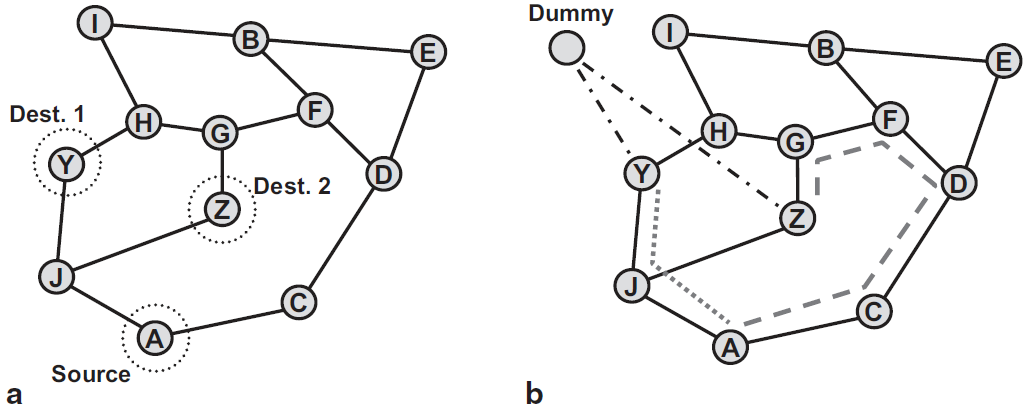
\includegraphics[width=140mm]{PSol6_Q1_2.png}
\end{figure}
\newpage
\Q

a. The following table shows the Dijkstra's algorithm steps:
\begin{figure}[h!]
\centering
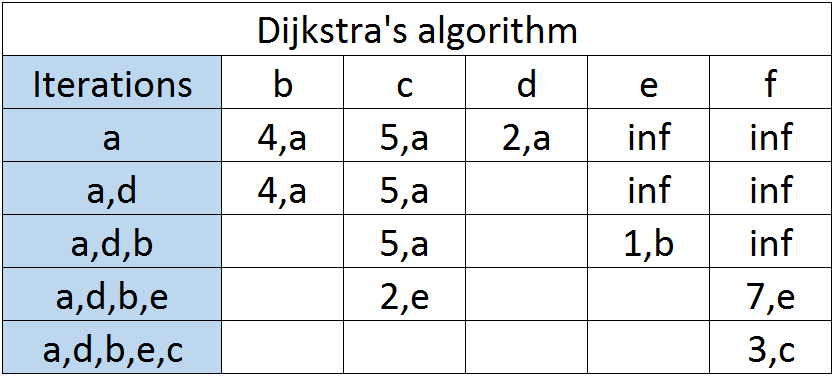
\includegraphics[width=140mm]{PSol6_Q2_1.png}
\end{figure}

As seen, the shortest path between nodes $a$ and $b$ is not optimum as the path $a-c-e-b$ has less cost.
\nl
b. The following table shows the Bellman-Ford's algorithm steps:
\begin{figure}[h!]
\centering
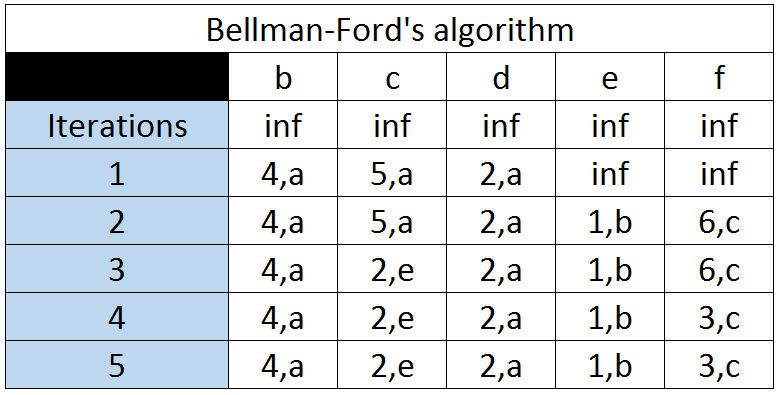
\includegraphics[width=140mm]{PSol6_Q2_2.png}
\end{figure}

Even still, the shortest path between nodes $a$ and $b$ is not optimum since the Bellman-Ford's algorithm does not yield to correct answer \textbf{when there is a negative cycle in the network.} The negative cycle in this case is the cycle $b-e-b$, as once a packet ariiving there, can be bounced back and forth between these two nodes two reduce the path cost to any arbitrarily low value.
\nl
c. The minimum-cost path is $a-b-e-f$, however by elevating the link costs by 2, we have the following altered version of the network:
\begin{figure}[h!]
\centering
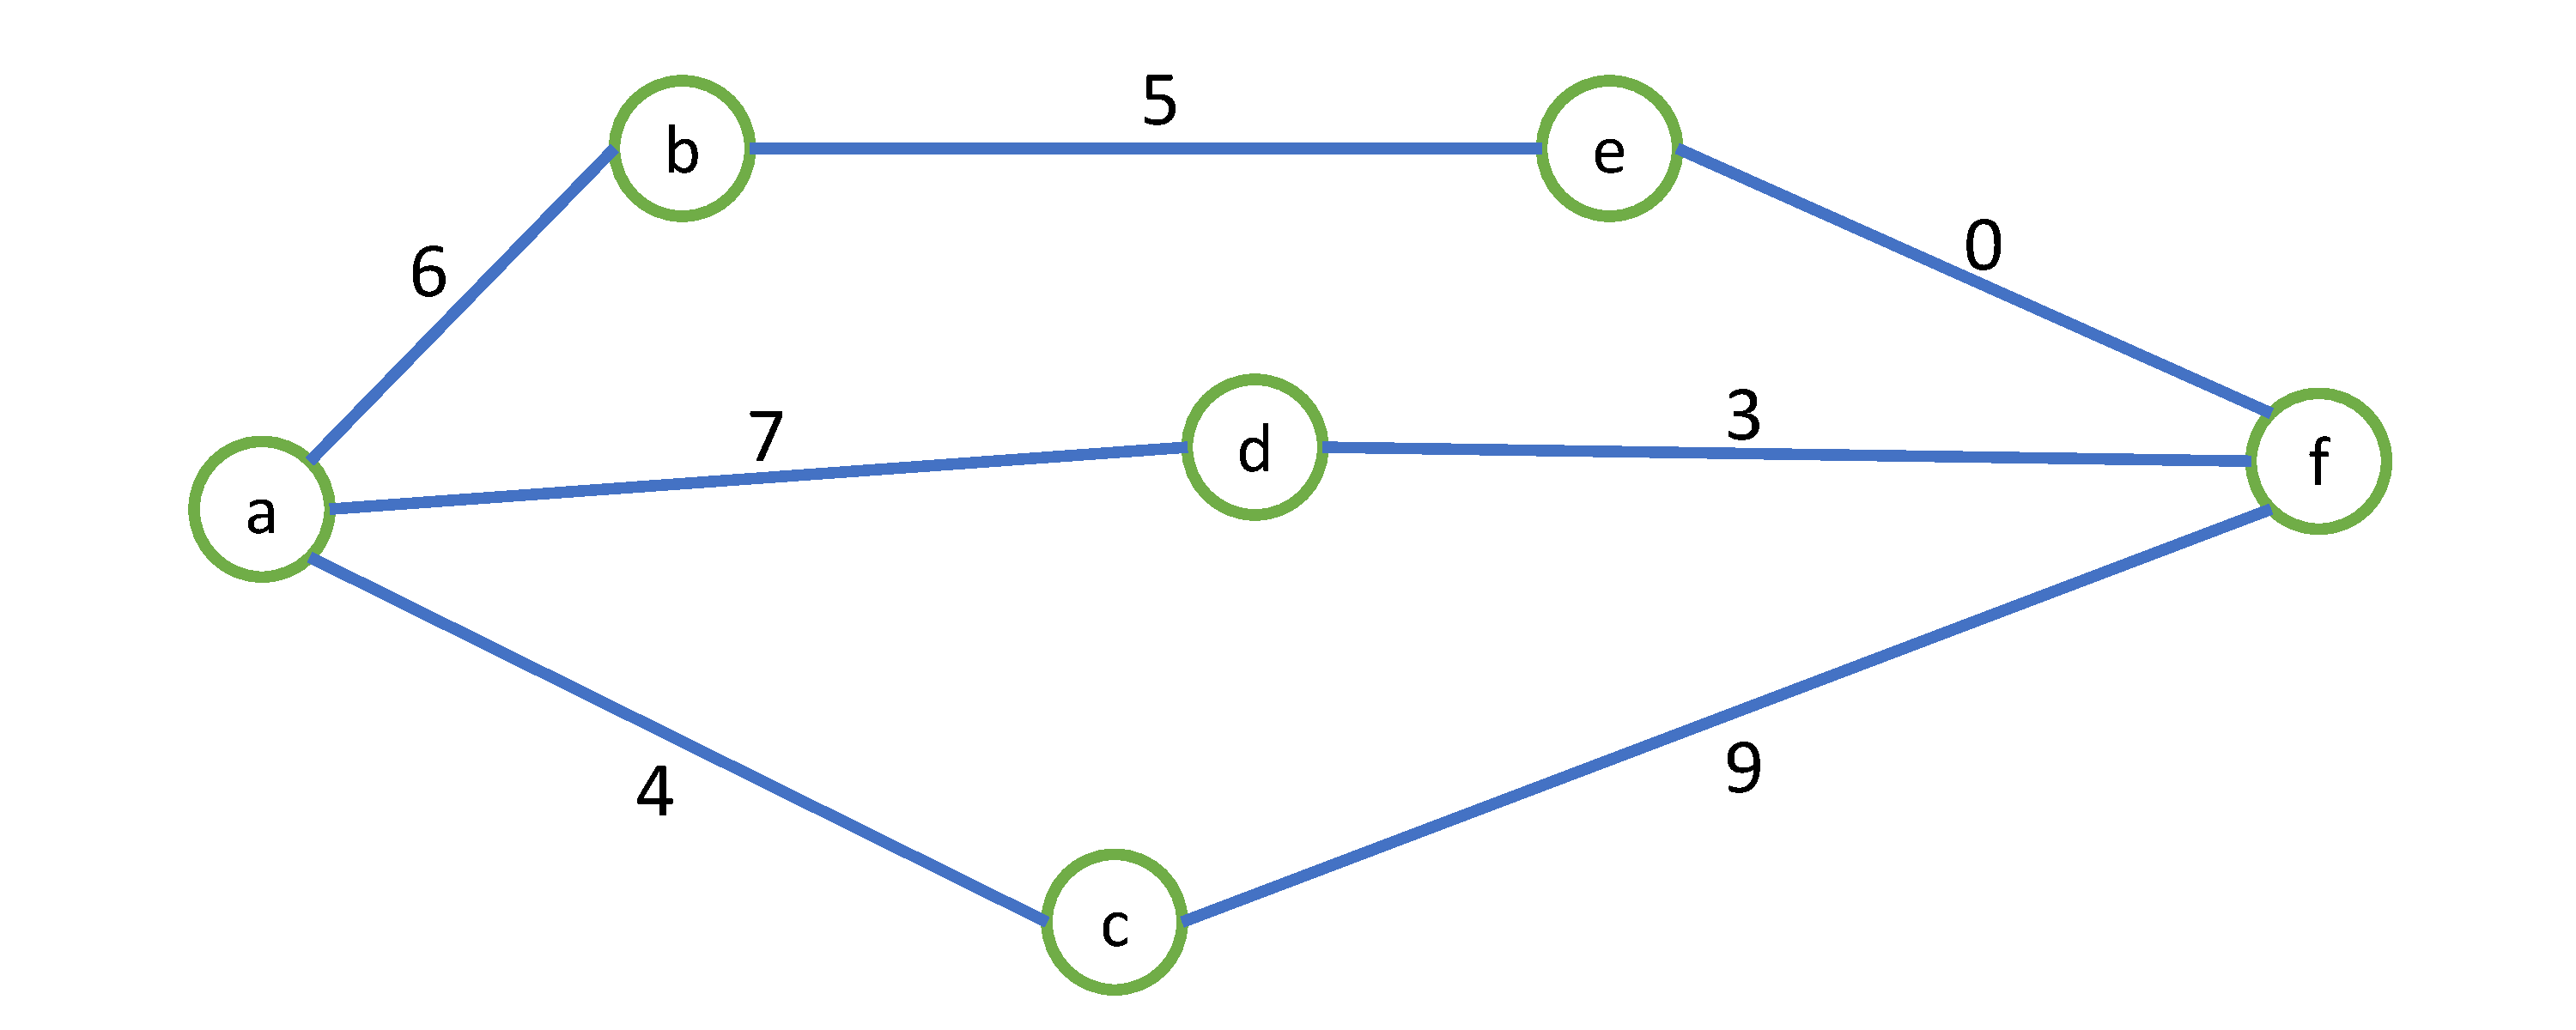
\includegraphics[width=140mm]{PSol6_Q2_3.pdf}
\end{figure}

with the new shortest path being $a-d-f$, which is actually incorrect.
\nl
\Q

We first sketch the feasible region of the optimization problem:
\begin{figure}[h!]
\centering
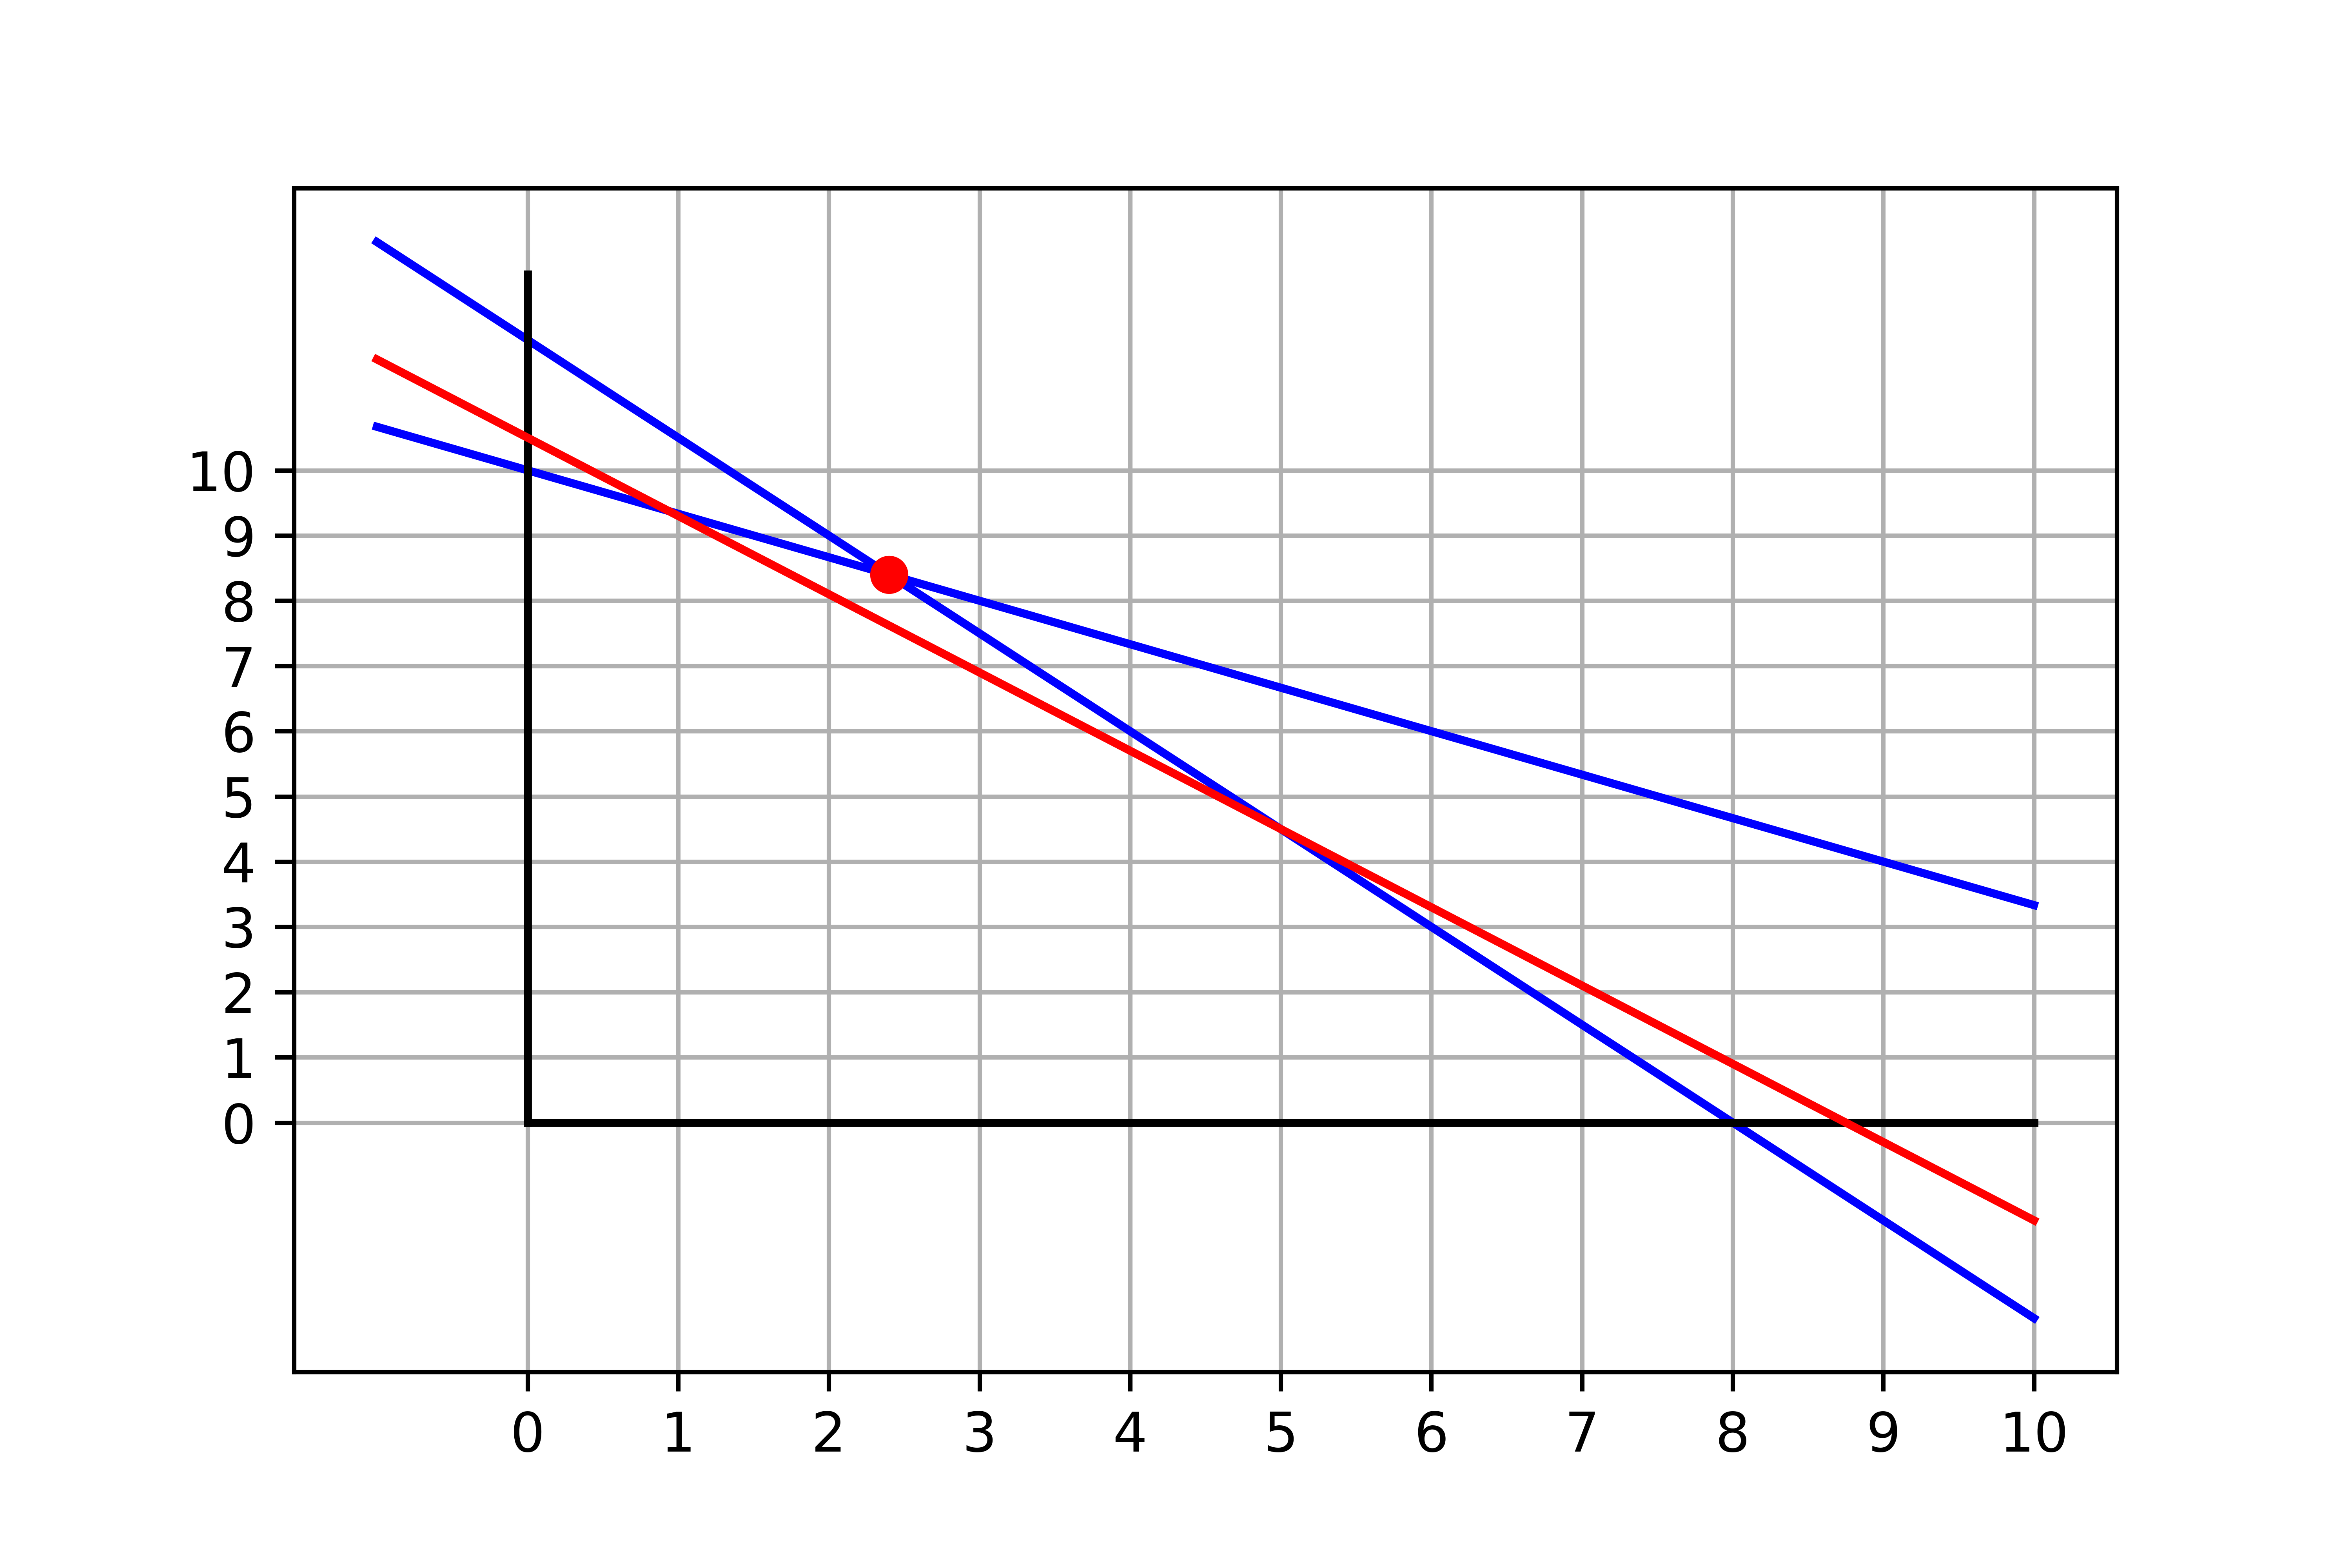
\includegraphics[width=140mm]{PSol6_Q3.png}
\end{figure}
Considering the gradient vector of the objective function, the red-marked point (where the two linear constraints meet), is the optimum solution to the optimization problem \textbf{when the variables are not constrained to be integers.} The point is $(2.4,8.4)$, so the ILP optimum solution can one of the following:
\qn{
&(2,8)
\\&(3,8)
\\&(2,9)
\\&(3,9)
}{}
Only the points $(2,8)$ is feasible which leads to the optimum value of 104.
\nl
\Q

The shortest paths can be calculated without considering the link capacities.
\qn{
&\text{Shortest path between 1 and 6} : 1-4-3-5-6
\\&\text{Shortest path between 2 and 6} : 2-3-5-6
}{}
\nl
\Q

a. Bhandari's algorithm:
\begin{figure}[h!]
\centering
\begin{subfigure}{0.49\textwidth}
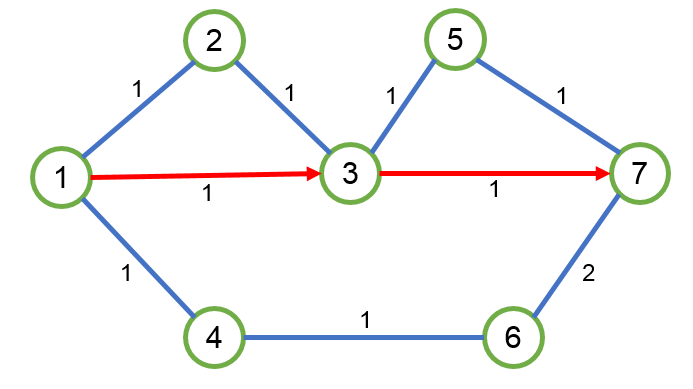
\includegraphics[width=80mm]{PSol6_Q5_1.png}
\end{subfigure}
\begin{subfigure}{0.49\textwidth}
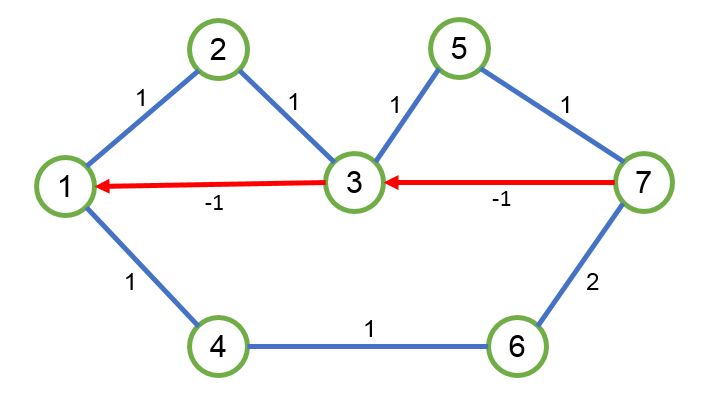
\includegraphics[width=80mm]{PSol6_Q5_2.png}
\end{subfigure}
\begin{subfigure}{0.49\textwidth}
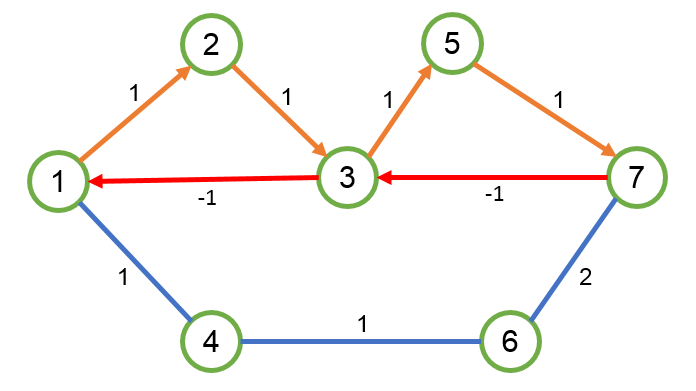
\includegraphics[width=80mm]{PSol6_Q5_3.png}
\end{subfigure}
\begin{subfigure}{0.49\textwidth}
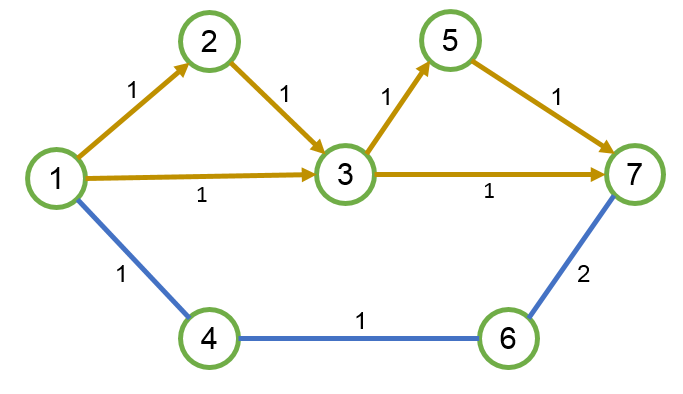
\includegraphics[width=80mm]{PSol6_Q5_4.png}
\end{subfigure}
\end{figure}
\newpage
b. Suurballe's algorithm:
\begin{figure}[h!]
\centering
\begin{subfigure}{0.49\textwidth}
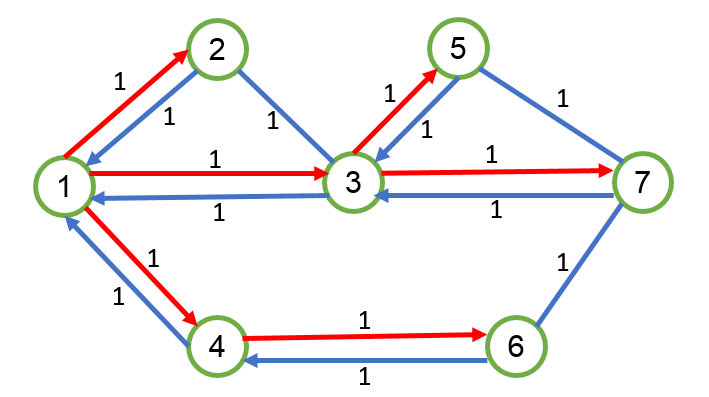
\includegraphics[width=80mm]{PSol6_Q5_5.png}
\end{subfigure}
\begin{subfigure}{0.49\textwidth}
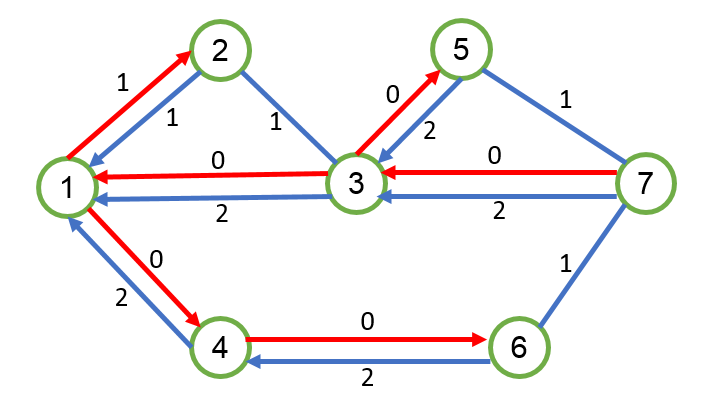
\includegraphics[width=80mm]{PSol6_Q5_6.png}
\end{subfigure}
\begin{subfigure}{0.49\textwidth}
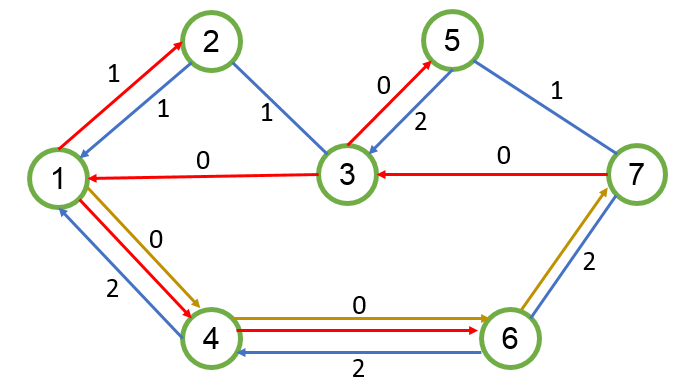
\includegraphics[width=80mm]{PSol6_Q5_7.png}
\end{subfigure}
\begin{subfigure}{0.49\textwidth}
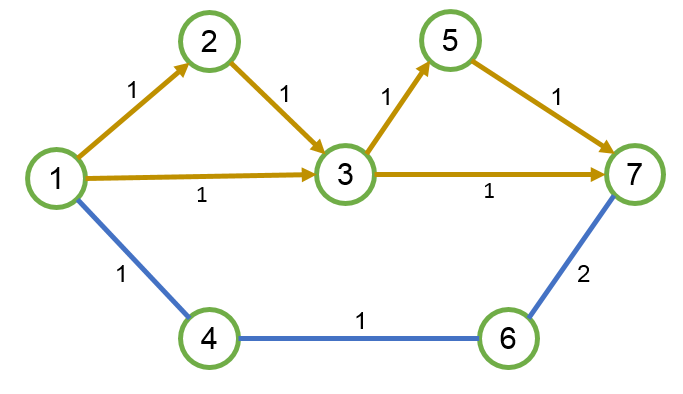
\includegraphics[width=80mm]{PSol6_Q5_4.png}
\end{subfigure}
\end{figure}

There two differences between Suurballe's and Bhandari's algorithm. Suurballe's algorithm relies on non-negative link costs and hence exploits the Dijkstra's algorithm while Bhandari's algorithm relies on generally valued link costs and hence exploits the Bellman-Ford's algorithm. Also Suurballe's algorithm leads to node disjoint paths while Bhandari's algorithm yields a link disjoint one.
\nl
\Q

By considering the following topology, we have included the SRLG in routing:
\begin{figure}[h!]
\centering
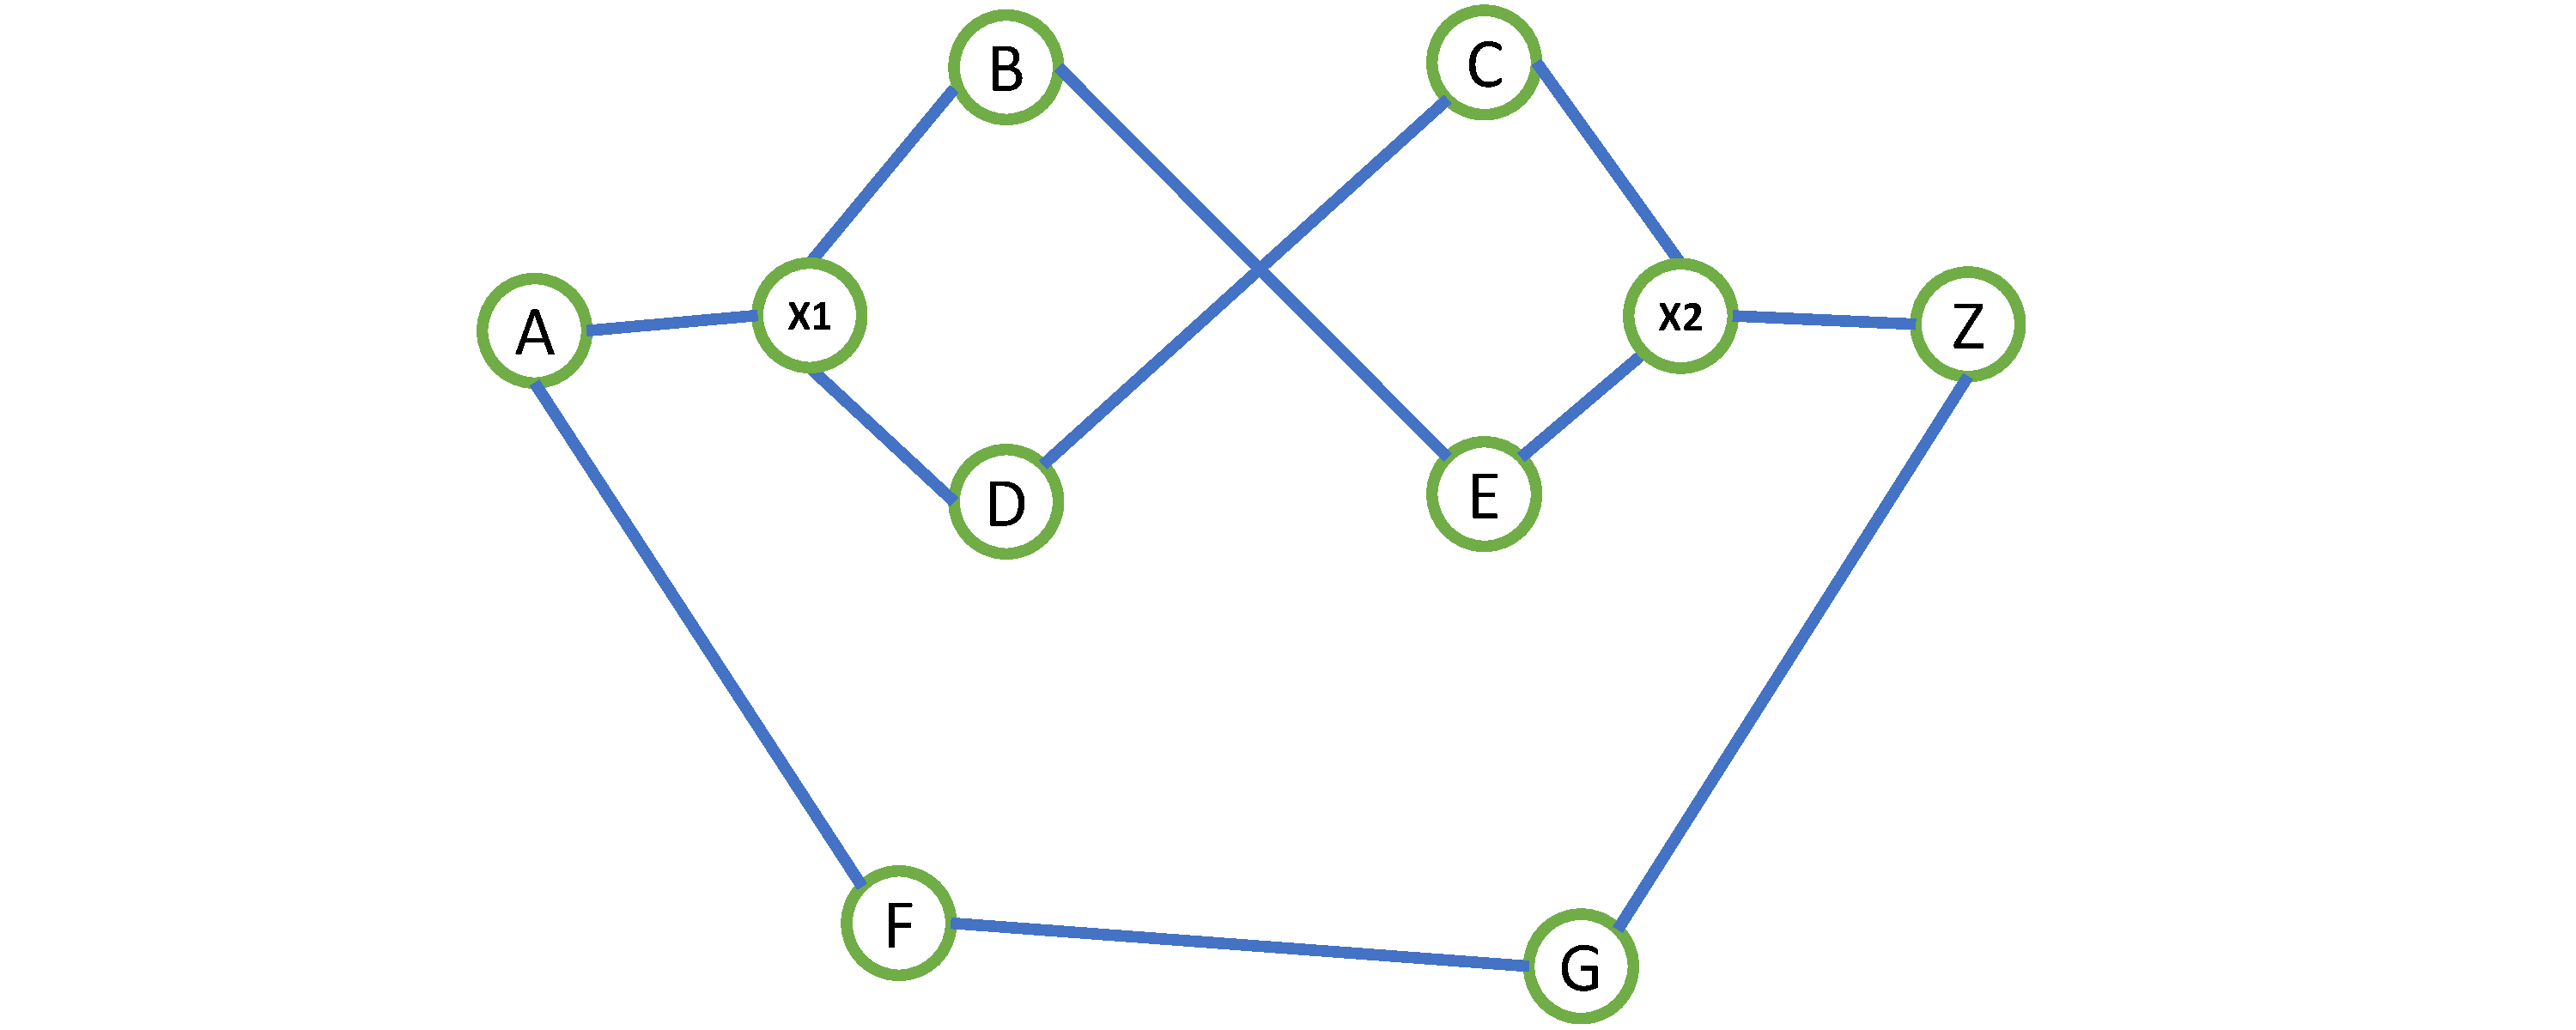
\includegraphics[width=160mm]{PSol6_Q6.pdf}
\end{figure}

The advantage of the new topology is that running a SPDP algorithm on the old network (where SRLG was not considered) may lead to link-disjoint paths A-B-E-Z and A-D-C-Z, however, in reality these two paths are not actually disjoint (a failure in the amplifer hut can bring down both the paths). In the new physical topology however, the possibility of co-existence of such paths is removed since the links A-X1 and X2-Z are now shared between such paths and as a consequence, the SPDP algorithms do not yield both the paths simultaneously.
\nl
\Q

In the first step, we extract a complete graph wose nodes are multicast group nodes and links denote the shortest paths between the corresponding nodes.
\begin{figure}[h!]
\centering
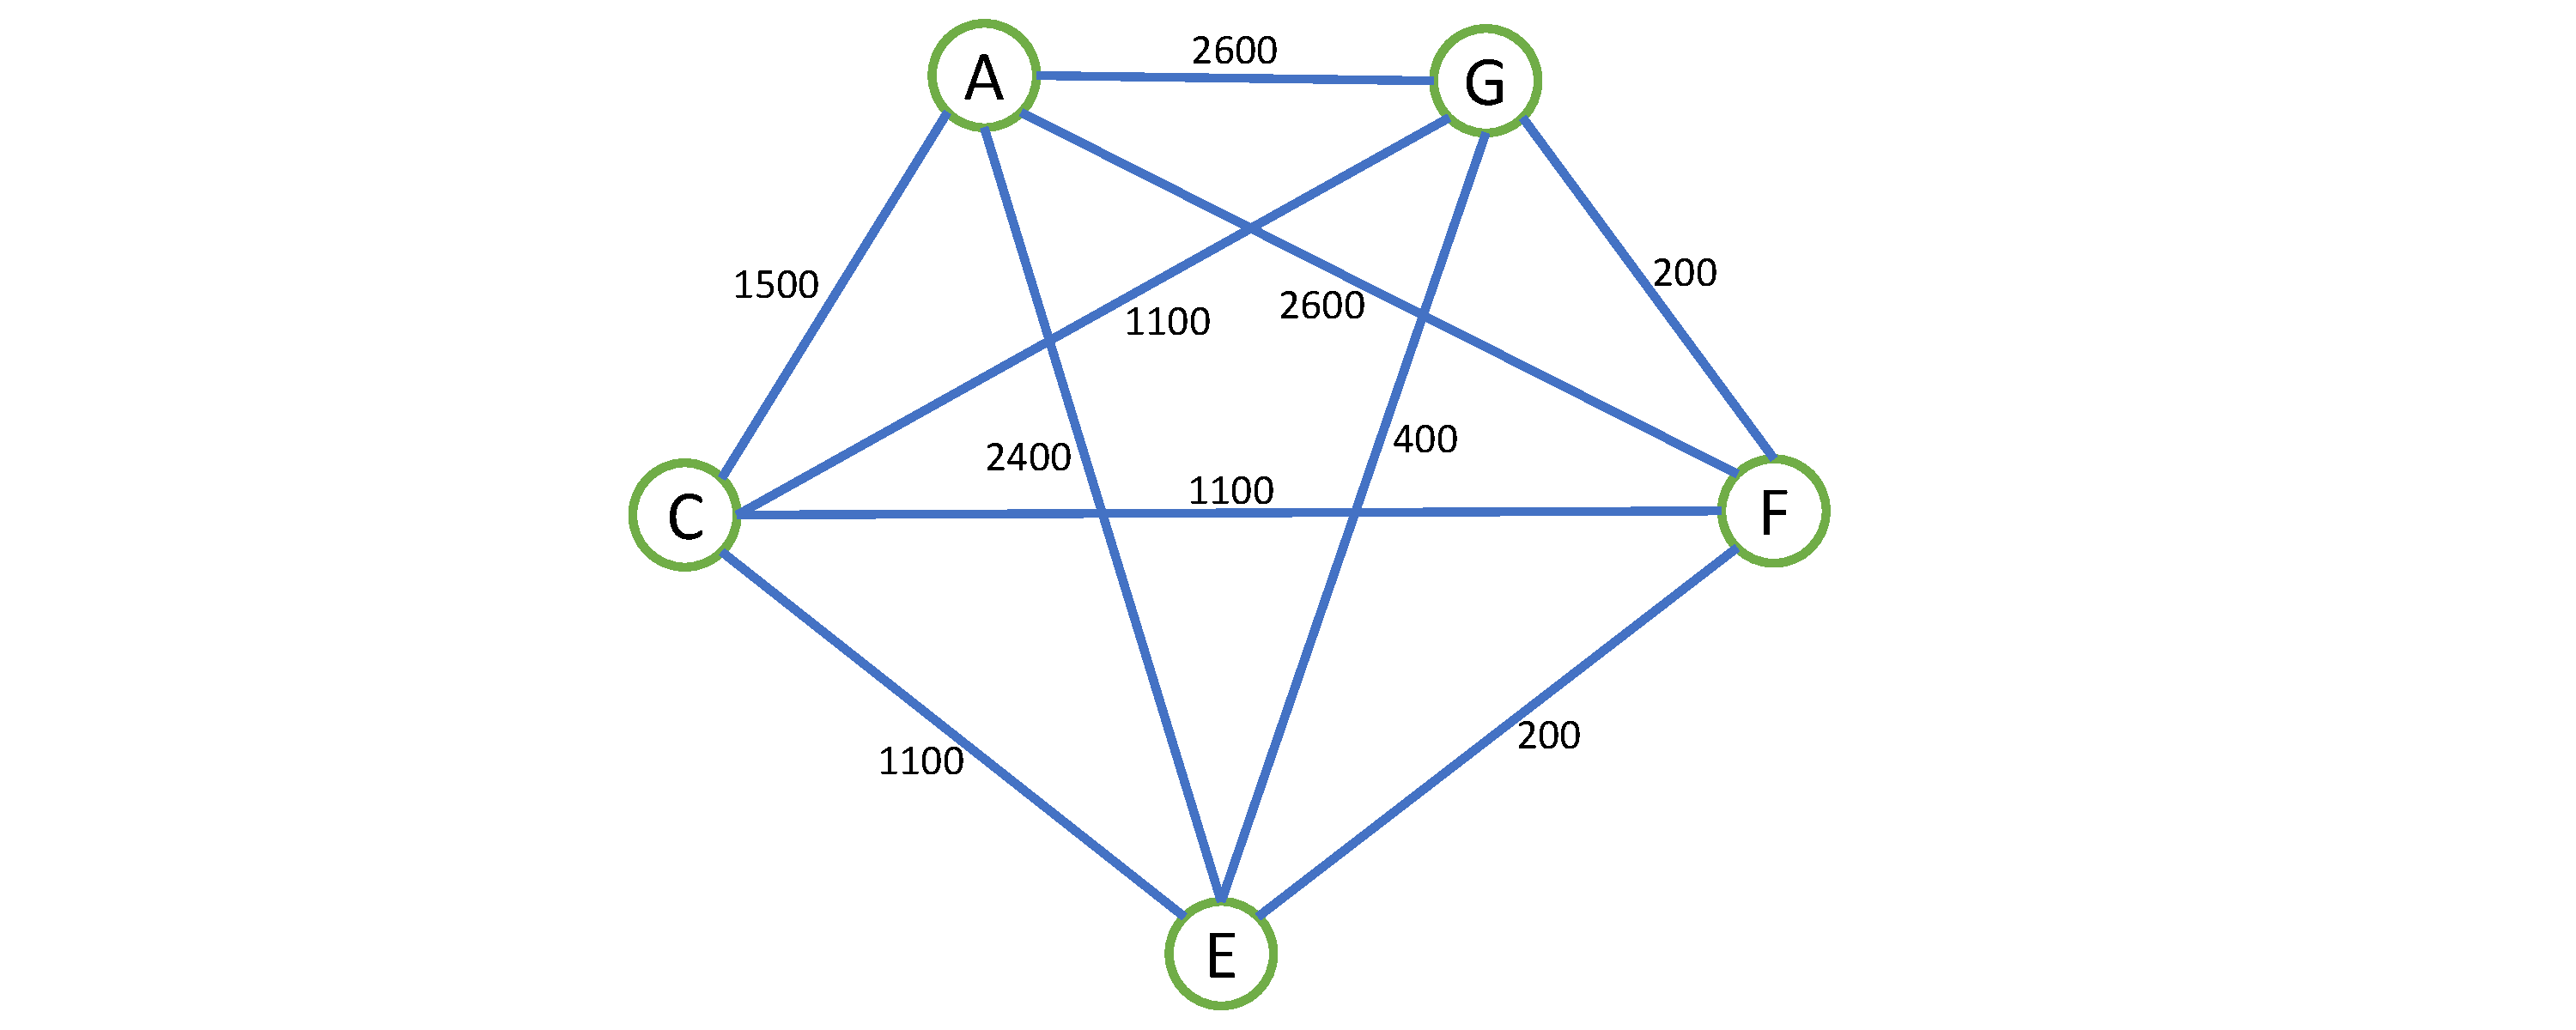
\includegraphics[width=160mm]{PSol6_Q7_1.pdf}
\end{figure}

Next, a minimum spanning tree is generated as:
\begin{figure}[h!]
\centering
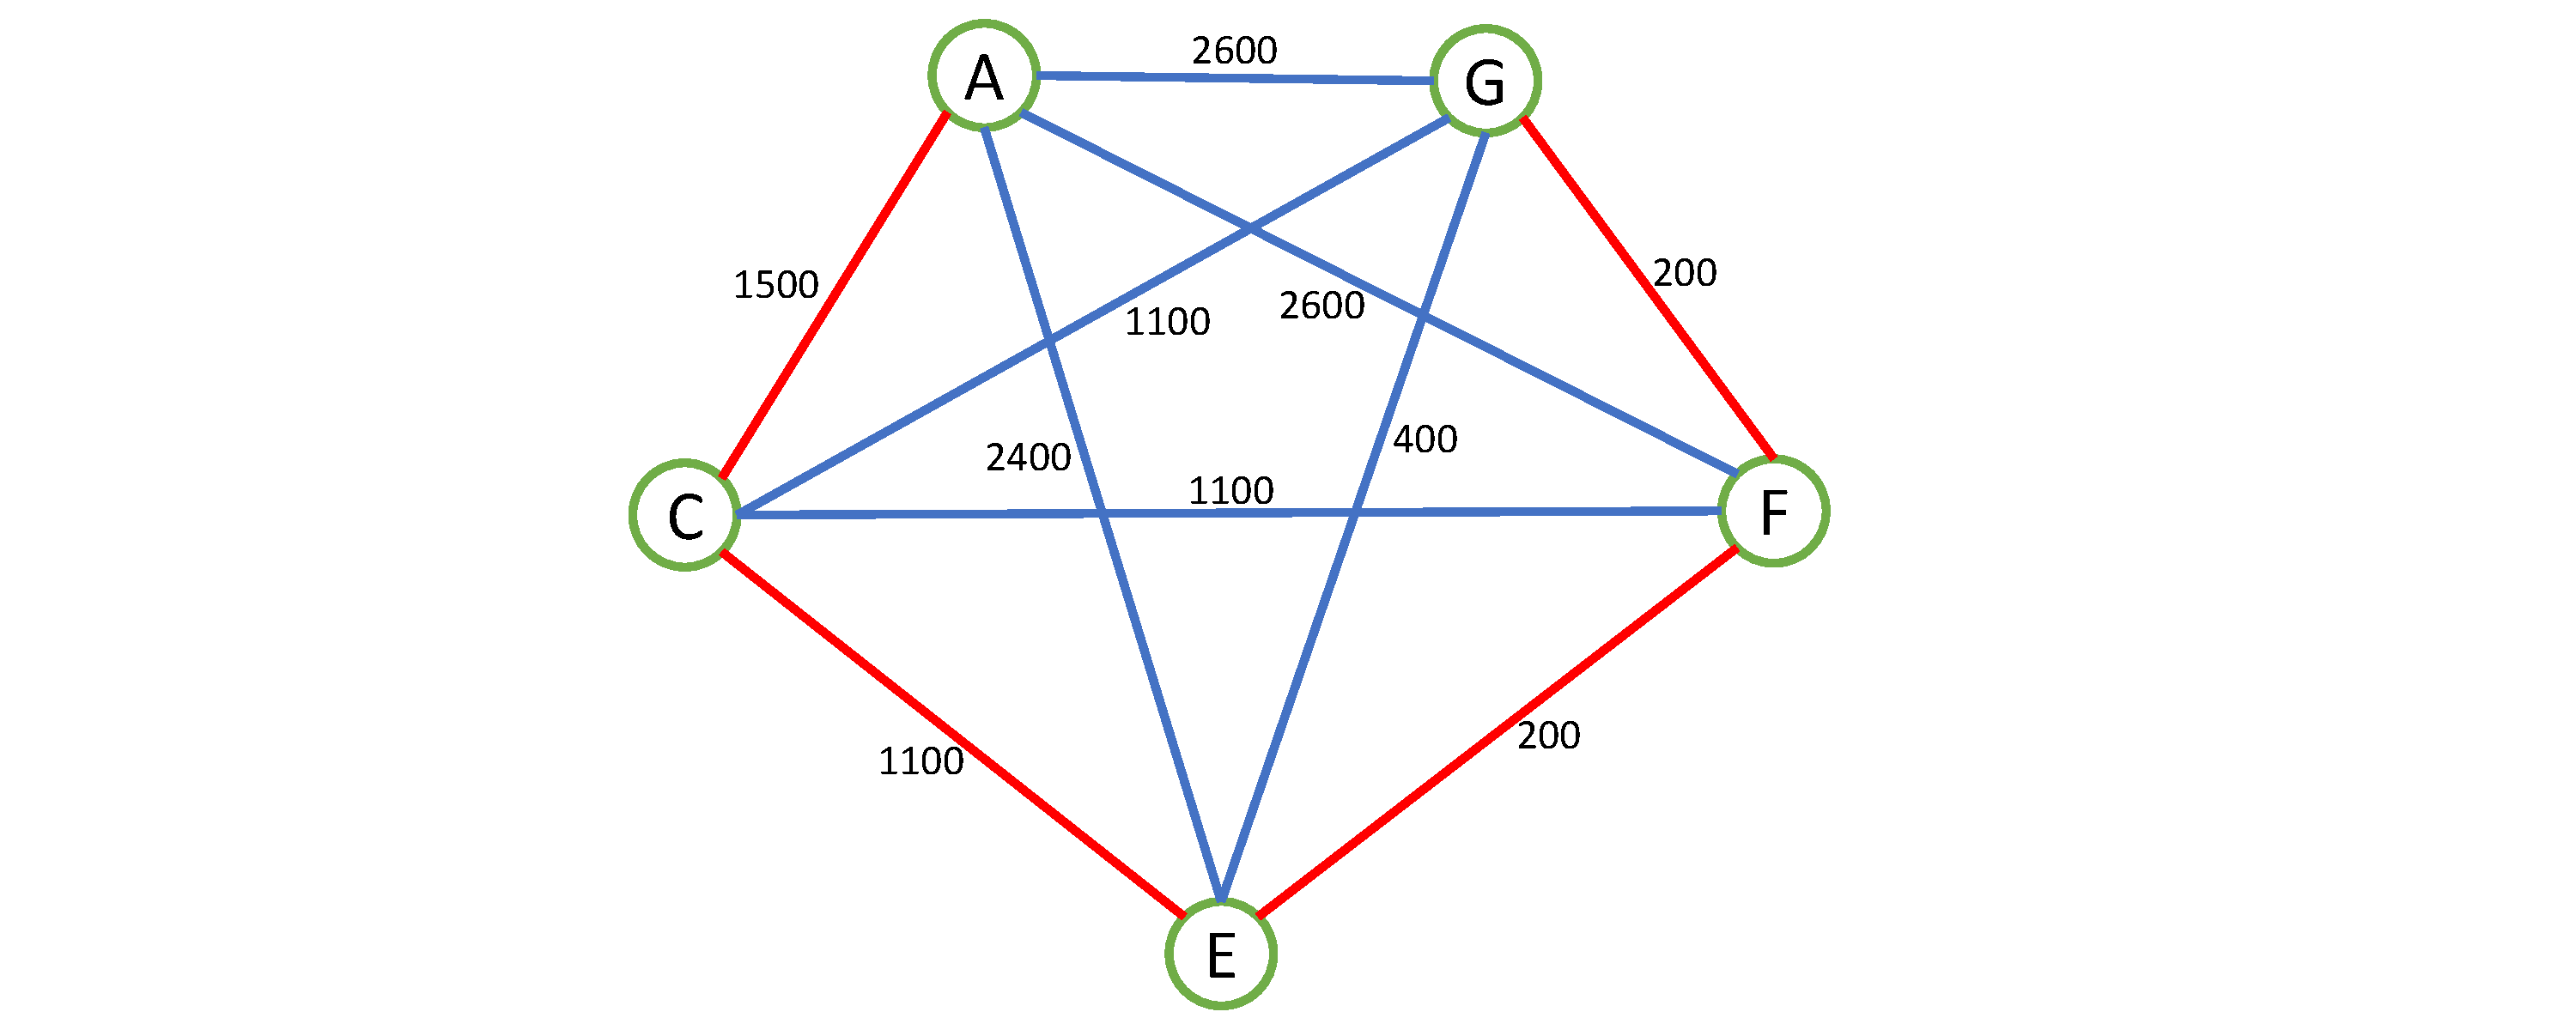
\includegraphics[width=160mm]{PSol6_Q7_2.pdf}
\end{figure}

Since all the shortest paths on the minimum spanning tree contain only multicast nodes (no non-multicast node such as B is included), the algorithm is terminated here and the found spanning tree is our final result.
\begin{figure}[h!]
\centering
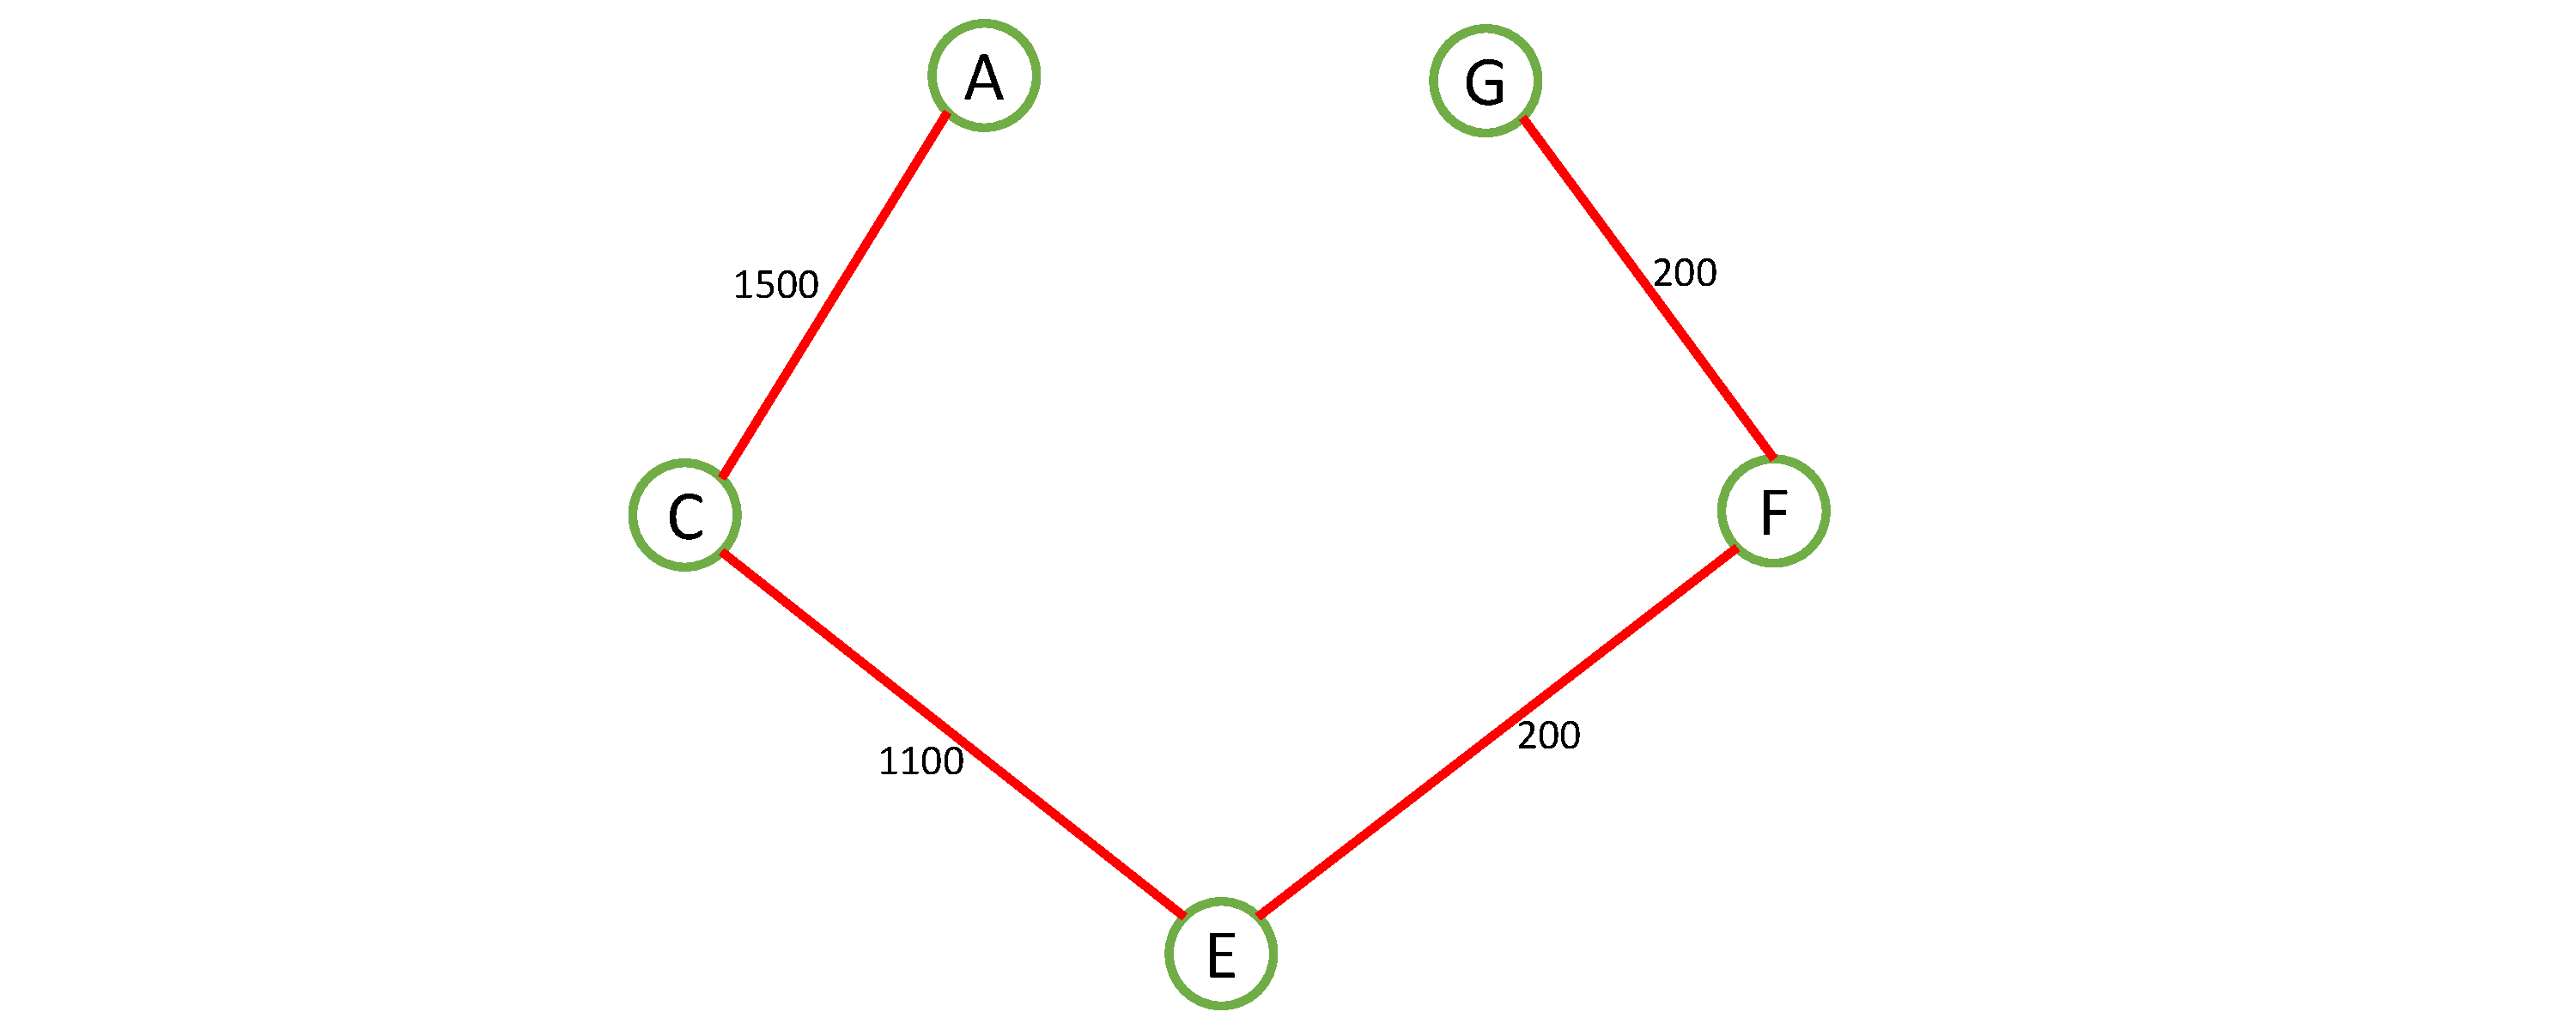
\includegraphics[width=160mm]{PSol6_Q7_3.pdf}
\end{figure}
%a. The RRC filter bandwidth is given by $(1+\beta)R_s$ where $\beta$ is the roll-off factor and $R_s$ is symbol rate. A simple substitution yields 36Gbaud.
%
%b. To sample a RRC filter with bandwidth 36G, we need to sample every 1/36 nsec ($f_{\text{Sampling}}$=36G) to avoid aliasing.
%
%c. Denote the uncoded bit stream by $b_n$. When passing through the \textbf{Bit-to symbol converter}, the stream turns into $s_n$ which is a sequence of symbols, e.g. each of which chosen from the alphabet $\{-1-j,-1+j,1-j,1+j\}$, hence the output becomes
%$$
%\sum_{n=-\infty}^{\infty} b_n\delta(t-nT_s)
%$$
%which has an inphase component of 
%$$
%\sum_{n=-\infty}^{\infty} \Re\{b_n\}\delta(t-nT_s)
%$$
%and a quadrature component of 
%$$
%\sum_{n=-\infty}^{\infty} \Im\{b_n\}\delta(t-nT_s)
%$$
%
%The upsampler is a system block for discretization considerations, and can be ignored since the discussion is fully taken place in analog regime. This leads to
%%$$
%%S(t)=\sum_{n=-\infty}^{\infty} b_n\delta(t-nT_s)
%%$$
%%Let's see what the Tx. output is. $S(t)$ passes through the \textbf{RRC pulse shaping block} which, as the name suggests, turns the ``impulse shape'' of the symbols in analog to ``RRC shape''. So far, the signal is constructed in baseband and is given by
%$$
%S(t)=\sum_{n=-\infty}^{\infty} \Re\{b_n\}s_\text{RRC}(t-nT_s)
%$$
%where $s_\text{RRC}(t)$ is the RRC pulse shape in time domain.
%
%The signal $S(t)$ is once multiplied in $\cos$ carrier and once in $\sin$ carrier to give the Tx. midband output signal as
%\qn{
%x(t)&=2\sum_{n=-\infty}^{\infty} \Re\{b_n\}s_\text{RRC}(t-nT_s)\cos 2\pi f_ct
%\\&-
%2\sum_{n=-\infty}^{\infty} \Im\{b_n\}s_\text{RRC}(t-nT_s)\sin 2\pi f_ct
%}{}
%which is directly input to Rx. block diagram based on back-to-back connection. The upper and lower branch signals after multiplying in $\cos$ and $-\sin$ become
%
%\qn{
%x(t)\cos 2\pi f_c t&=
%2\sum_{n=-\infty}^{\infty} \Re\{b_n\}s_\text{RRC}(t-nT_s)\cos^2 2\pi f_ct
%\\&-
%2\sum_{n=-\infty}^{\infty} \Im\{b_n\}s_\text{RRC}(t-nT_s)\sin 2\pi f_ct\cos 2\pi f_ct
%\\&=
%\sum_{n=-\infty}^{\infty} \Re\{b_n\}s_\text{RRC}(t-nT_s)(\cos 4\pi f_ct-1)
%\\&-
%\sum_{n=-\infty}^{\infty} \Im\{b_n\}s_\text{RRC}(t-nT_s)\sin 4\pi f_ct
%}
%and
%\qn{
%x(t)\sin 2\pi f_c t&=
%\sum_{n=-\infty}^{\infty} \Re\{b_n\}s_\text{RRC}(t-nT_s)\sin 4\pi f_ct
%\\&-
%\sum_{n=-\infty}^{\infty} \Im\{b_n\}s_\text{RRC}(t-nT_s)(1-\cos 4\pi f_ct)
%}
%The $\cos 4\pi f_ct$ and $\sin 4\pi f_ct$ are modulated by a baseband signal to midband frequency $2f_c$ and are not passed through the ideal low-pass filter. Hence the output of the filter is
%\qn{
%\text{Output of the LPF}=\sum_{n=-\infty}^{\infty} \Re\{b_n\}s_\text{RRC}(t-nT_s)
%}
%which turns into 
%$$
%Y(t)=\sum_{n=-\infty}^{\infty} \Re\{b_n\}s_\text{RC}(t-nT_s)
%$$
%after passing through the RRC matched filter (RRC pulse shape) block since
%$$
%s_\text{RRC}(t)*s_\text{RRC}(t)=s_\text{RC}(t)
%$$
%d. The above reasoning makes it clear as to why LPF is needed. We need LPF to extract the baseband signal out from a total received, midband signal since our pure information lays there.
%\nl
%\Q
%
%a. We have 4 inner points of power $1^2+1^2=2$, 8 points with power $1^2+3^2=10$ and 4 outer points with equal power $3^2+3^2=18$, all of which equally likely. Hence the average power is 
%$$
%{1\over 16}(4\times 2+8\times 10+4\times 18)=10
%$$
%
%b. The desired average power is assumed 6.8, which is
%$$
%2P_1+10P_2+10P_3+18P_4=6.8
%$$
%or equivalently
%$$
%24P_3+18P_4=6.8
%$$
%also
%$$
%P_1+P_2+P_3+P_4=1\implies 4P_3+P_4=1
%$$
%with the following solution
%\qn{
%&P_1=0.47
%\\&P_2=0.23
%\\&P_3=0.23
%\\&P_4=0.07
%}
%\Q
%
%a. Each 4 bits of an input stream are mapped to a symbol in 16QAM, leading to a bit rate of 96 Gbps.
%
%b. Since the channel encoder adds redundant bits to the input bit stream, each 3 input bits are mapped to 4 bits, thereby yielding a total bit rate of
%$$
%96\times {4\over 3} Gbps=128 Gbps
%$$
%c.
%$$
%96\times {6\over 5} Gbps=115.2 Gbps
%$$
%which is less than that in part b- since the redundancy is decreased.
%
%d. For unshaped 8QAM and 32QAM, the bit-to-symbol conversion ratio is 3 and 5, respectively, hence
%\qn{
%&\text{8QAM uncoded bit rate}=24\times 3=72Gbps
%\\&
%\text{32QAM uncoded bit rate}=24\times 5=120Gbps
%}
%similarly
%\qn{
%&\text{8QAM encoded bit rate}=24\times 3=86.4Gbps
%\\&
%\text{32QAM encoded bit rate}=24\times 5=144Gbps
%}
%e. The bit-to-symbol ratio can be calculated from 
%$$
%H=-\sum_{i=1}^{16} \hat P_i\log_2 \hat P_i
%$$
%which with the probabilisitic shaping parameters calculated in question 2, gives 
%$$
%H=3.76 \text{ bits}
%$$
%f. The bit rate is correspondingly equal to $24 G\times 3.76=90.24 \text{ Gbps}$, which when encoded, increases by ${6\over 5}$ to $108.29\text{ Gbps}$, though less than $115.2 Gbps$ since the number of bits per symbol is reduced.
%\nl
%\Q
%
%a and b. The ASE power spectral density is
%\qn{
%\sigma^2_\text{ASE,PSD}={1\over 2}N_\text{Span}h\nu_\text{opt} GF=16.06\mu\text{W/Gbaud}
%}
%hence the ASE noise variance becomes
%\qn{
%\sigma^2_\text{ASE}&=R_\text{Receiver}\sigma^2_\text{ASE,PSD}\\&=
%(1+\beta)R_s\sigma^2_\text{ASE,PSD}\\&=0.462 \text{mW}\equiv -3.35 \text{dBm}
%}{}
%and the SNR is calculated as
%$$
%\text{SNR (dB)}=\text{Power (dBm)}-\sigma^2_{ASE}\text{ (dBm)}=12.75 \text{dB}
%$$
%c. A LDPC code with parameters (16193,9713) is needed to obtain a probability of error as $\sim 2\times 10^{-3}$. With such probability of error, a RS code with parameters (294,244) can reduce the probability of error by an astounding factor to $10^{-10}$.
%
%d. That probabilistic shaping reduces the launch power by 32\% and hence the SNR; therefore
%$$
%\text{SNR}_{\text{Shaped}}=11.08\text{ dB}
%$$
%with an approximate probability of error of $\sim 5\times 10^{-3}$. Similarly, the LDPC and RS code parameters are (16195,12595) and (294,244) and the reduced probability of error is $\sim 10^{-6}$, respectively.
\end{document}